\documentclass[tikz]{standalone}
\usetikzlibrary{intersections}
\begin{document}
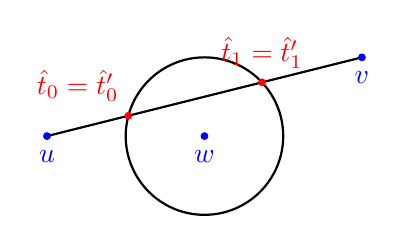
\begin{tikzpicture}
  \coordinate (u) at (0,0);
  \coordinate (v) at (4,1);
  \coordinate (w) at (2,0);

  \draw[thick] (u) -- (v);
  \draw[thick] (w) circle (1);

  \path[name path=line] (u) -- (v);
  \path[name path=circle] (w) circle (1);
  \path[name intersections={of=line and circle, by={t1,t0}}];

  \node[circle,fill,color=blue,inner sep=1pt,label={[text=blue]-90:\(u\)}] at (u) [] {}; 
  \node[circle,fill,color=blue,inner sep=1pt,label={[text=blue]-90:\(v\)}] at (v) [] {}; 
  \node[circle,fill,color=blue,inner sep=1pt,label={[text=blue]-90:\(w\)}] at (w) [] {}; 

  \node[circle,fill,color=red,inner sep=1pt,label={[text=red, above left]:\(\hat t_0=\hat t_0'\)}] at (t0) [] {}; 
  \node[circle,fill,color=red,inner sep=1pt,label={[text=red, above]:\(\hat t_1=\hat t_1'\)}] at (t1) [] {}; 
\end{tikzpicture}
\end{document}
